\documentclass[prez_parietal.tex]{subfiles}
\begin{document}


\begin{frame}{D-step: solving for the atoms}

The dictionary update is performed by minimizing
\begin{equation}
\min_{\|d_{k}\|_2 \leq 1} E(\{d_k\}_k) \overset{\Delta}{=} \sum_{n=1}^N\frac{1}{2}\|X^n - \sum_{k=1}^K z^n_k * d_k\|_{2}^{2} \hspace{6pt}
\enspace .
\end{equation}

Computing $\nabla_{d_k} E(\{d_k\}_k)$ can be done efficiently
\[
\nabla_{d_{k}} E(\{d_k\}_k)
= \sum_{n=1}^N (z_k^n)^\Lsh * \left(x^n - \sum_{l=1}^K z^n_l * d_l\right)
=  \Phi_k - \sum_{l=1}^K \Psi_{k, l} *  d_l \enspace ,
\]

\strongpoint{Save with Projected Gradient Descent (PGD) with an Armijo backtracking line-search for the d-step \mycite{Wright1999}.}

\end{frame}




\begin{frame}{How to extend CSC to multivariate signals?}
We can just use multivariate convolution,
\[
\underbrace{X[t]}_{\in\Rset^P} = \sum_{k=1}^K \left(z_k * \pmb D_k\right)[t] = \sum_{k=1}^K \sum_{\tau=1}^L z_k[t-\tau] \underbrace{\pmb D_k[\tau]}_{\in \Rset^P}
\]
with:
\begin{itemize}
\item $X$ a multivariate signal of length $T$ in $\Rset^P$
\item $\pmb D_k$ a multivariate signal of length $L$ in $\Rset^P$
\item $z_k$ a univariate activation signal of length $\widetilde{T} = T - L + 1$
\end{itemize}
\vskip1em
However, this model does not account for the physics of the problem.
\end{frame}

\begin{frame}{EM wave diffusion}
\begin{itemize}
\uncover<1->{\item Recording here with 8 sensors}
\uncover<2->{\item EM activity in the brain}
\uncover<3->{\item The electric field is spread \textbf{linearly} and \textbf{instantaneously} over all sensors (Maxwell equations)}
\end{itemize}
\centering
\only<1>{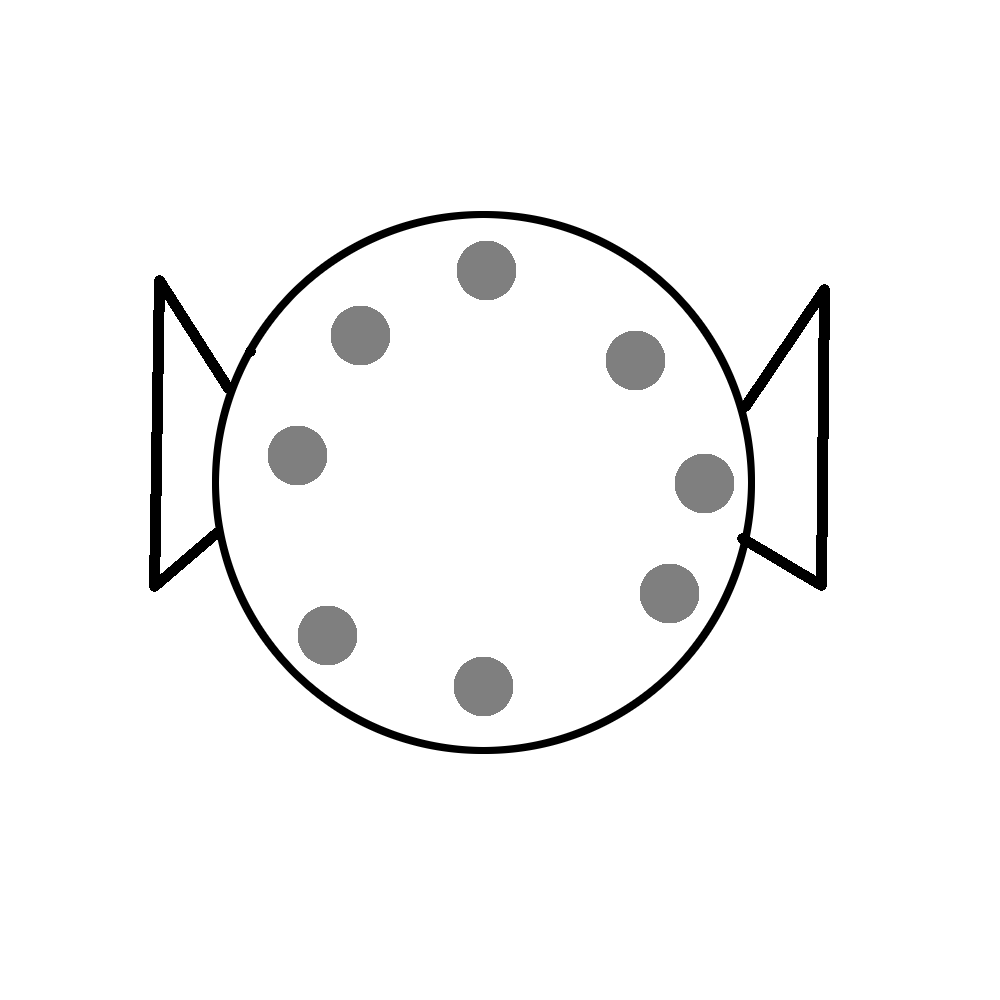
\includegraphics[width=.5\textwidth]{physic1}}%
\only<2>{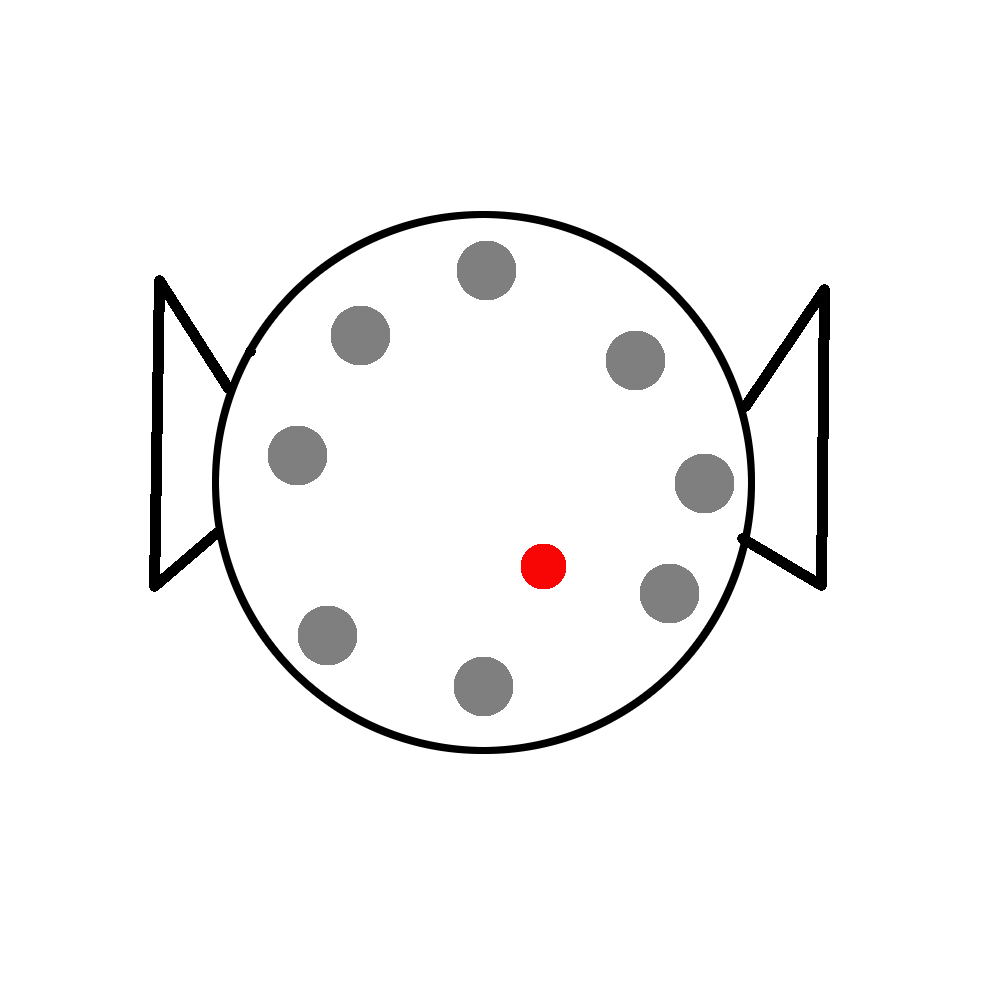
\includegraphics[width=.5\textwidth]{physic2}}%
\only<3>{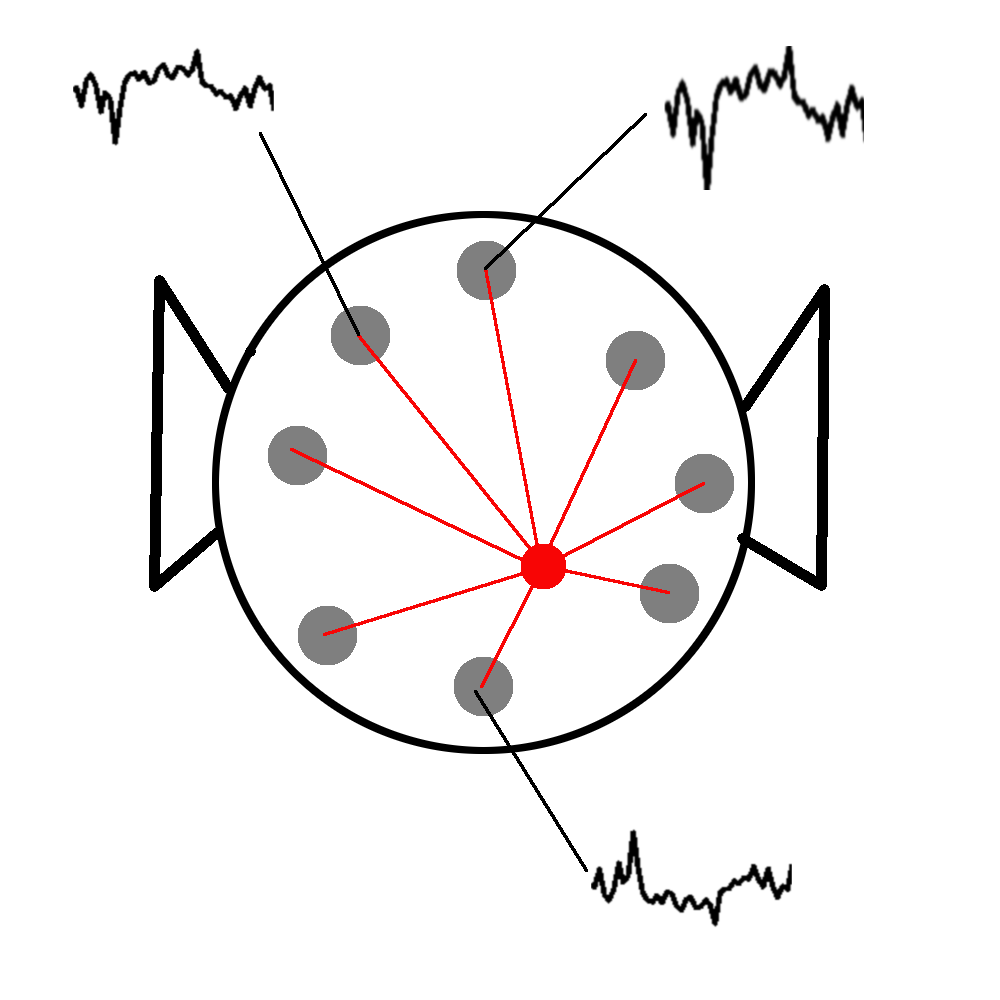
\includegraphics[width=.5\textwidth]{physic3}}
\end{frame}

\begin{frame}{Multivariate CSC with rank-1 constraint}
\textbf{Idea}: Impose a rank-1 constraint on the dictionary atoms $D_k$
\vskip1em
To make the problem tractable, we decided to use auxiliary variables $u_k$ and $v_k$ \st{} $D_k = u_kv_k\top$.

\begin{equation}
\label{eq:multichannel_csc}
\begin{split}
\min_{u_k, v_k, z_k^n} &\sum_{n=1}^N\frac{1}{2}\left\|X^n - \sum_{k=1}^K z^n_k * (u_k^{ } v_k^\top)\right\|_{2}^{2}
+ \lambda  \sum_{k=1}^K \left\|z^n_k\right\|_1, \hspace{6pt}\\
&\text{s.t. } ~~ \|u_{k}\|_2^2 \leq 1 \text{  , }\|v_{k}\|_2^2 \leq 1 \text{  and } z_k^n \geq 0~.
\end{split}
\end{equation}

Here,
\begin{itemize}
\item $u_k \in \Rset^P$ is the spatial pattern of our atom
\item $v_k \in \Rset^L$ is the temporal pattern of our atom
\end{itemize}
\end{frame}

\begin{frame}{Update in $u_k$ and $v_k$}

The problem is not jointly convex in $u_k$ and $v_k$.\\[1em]
Use an alternate minimization on these two blocks.\\[2em]

The gradient can also be computed using sufficient statistics $\phi$ and $\psi$:
\[
\begin{split}
\nabla_{u_k} E(\{u_k\}_k, \{v_k\}_k) &=  \nabla_{D_k}E(\{u_k\}_k, \{v_k\}_k) v_k
~~ \in \Rset^{P}~,\\
\nabla_{v_k} E(\{u_k\}_k, \{v_k\}_k) &=  u_k^\top \nabla_{D_k} E(\{u_k\}_k, \{v_k\}_k) 
~~ \in \Rset^L~,
\end{split}
\]
\end{frame}

\begin{frame}{Fast optimization}
Comparison with multivariate methods on somato dataset with $T=134,700$, $K=8$, $P=5$ and $L=128$\\[1em]
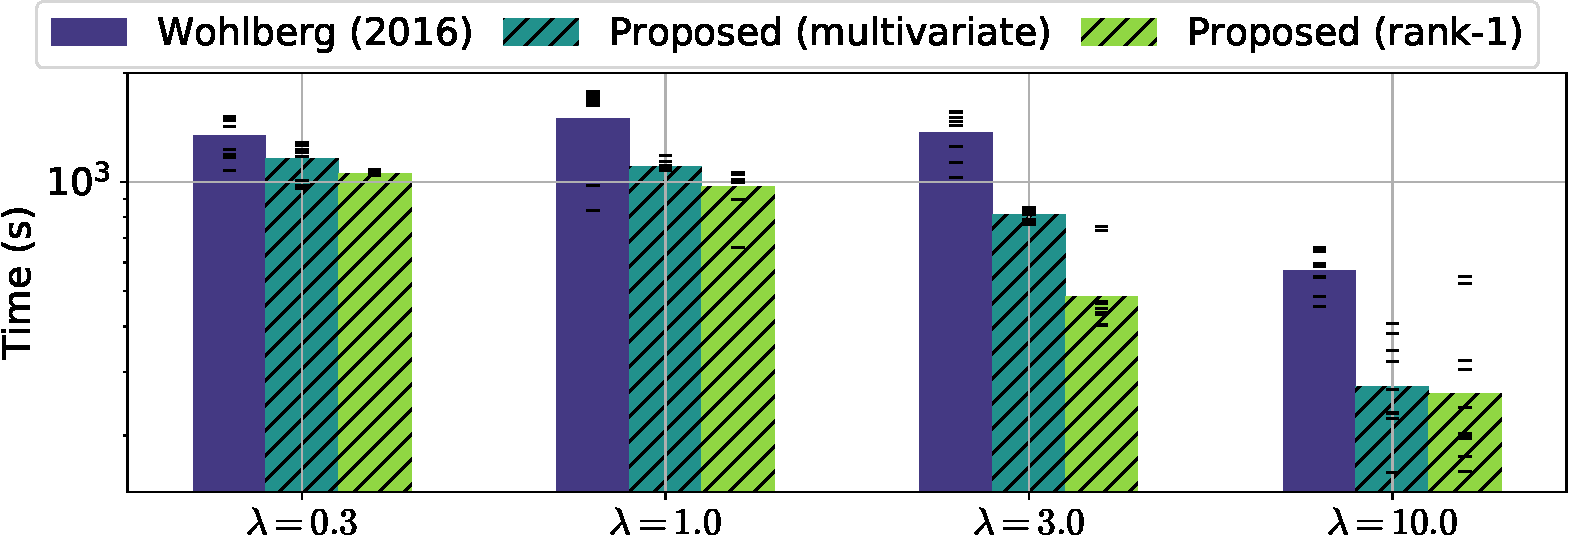
\includegraphics[width=\textwidth]{all_last_0001_T_13470_P5_K8_L128}
\end{frame}


\begin{frame}{Pattern recovery}
Patterns recovered with $P = 1$ and $P=5$. The signals were generated with the two simulated temporal patterns and with  $\sigma = 10^{-3}$. \\[1em]
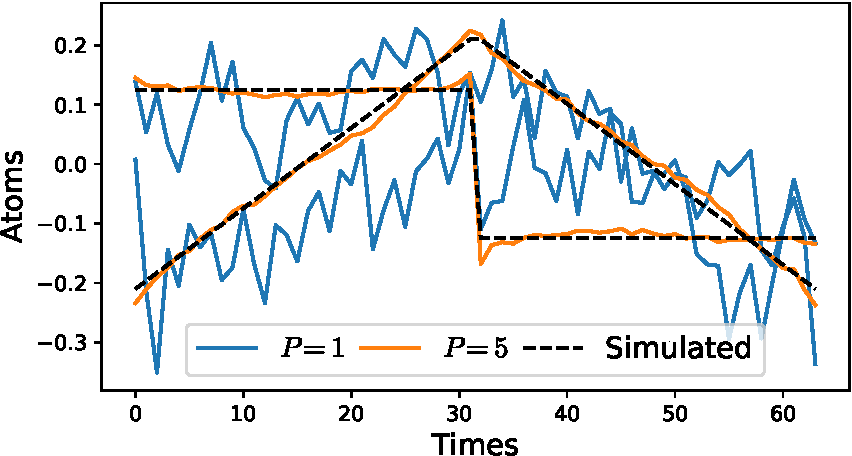
\includegraphics[width=\textwidth]{1D_vs_multi_uv_hat_P5.pdf}
\end{frame}
\begin{frame}{Pattern recovery}
Evolution of the recovery loss with $\sigma$ for different values of $P$. Using more channels improves the recovery of the original patterns.\\[1em]
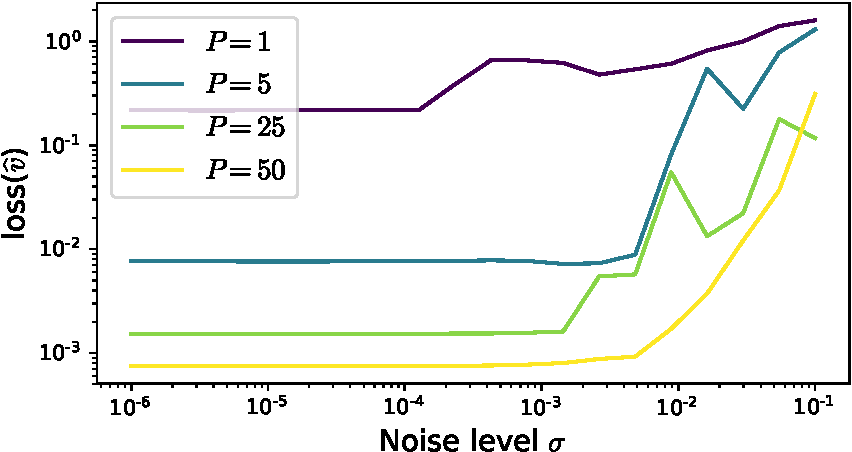
\includegraphics[width=\textwidth]{1D_vs_multi.pdf}
\end{frame}


\section{Experiments on Real Dataset}
\begin{frame}[t]
\vskip5em
\centering
\begin{beamercolorbox}[sep=8pt,center,shadow=true,rounded=true]{title}
\usebeamerfont{title}\insertsectionhead%
\end{beamercolorbox}
\vskip5em
\flushleft
\large Good time to wake-up if you got lost in the previous section!
\end{frame}

\begin{frame}{MNE somatosensory data}
A selection of temporal waveforms of the atoms learned on the MNE sample dataset.\\
\centering
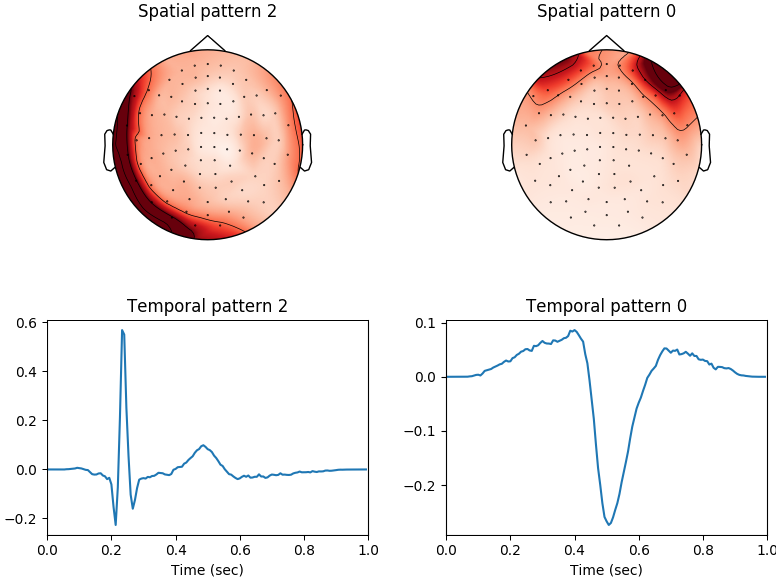
\includegraphics[height=0.8\textheight]{artifacts}
\end{frame}


\begin{frame}{MNE somatosensory data}
Atoms revealed using the MNE somatosensory data. Note the non-sinusoidal comb shape of the mu rhythm.\\[1em]
\centering
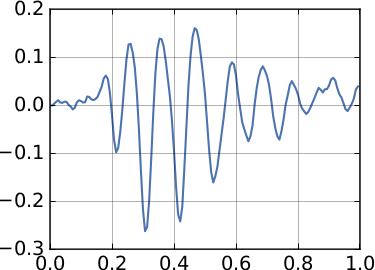
\includegraphics[height=.35\textheight]{atoms_somato_a.png}\hskip3em
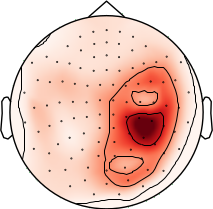
\includegraphics[height=.35\textheight]{atoms_somato_b.png}\\[.3em]\hskip1em
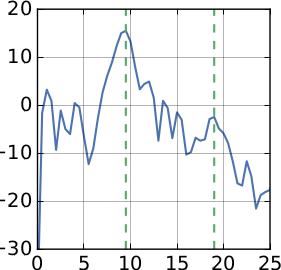
\includegraphics[height=.35\textheight]{atoms_somato_c.png}\hskip3em
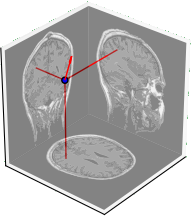
\includegraphics[height=.35\textheight]{atoms_somato_d.png}
\end{frame}
    
\end{document}